\section{Introduction}

Data, curated by journalists, scientists and policy makers into charts and other visual summaries, is how we understand the changing world around us. But charts can be hard to interpret correctly, even with access to the relevant data source. Innocent (but devastating) mistakes such as transposing two columns of data may go unnoticed for several years, even in widely cited papers~\cite{miller06}. Less innocent mistakes are deployed by politicians to mislead voters \cite{fullfact19}. Making sense of (and trusting) a visualisation, even for an expert, means understanding what its visual attributes actually \emph{represent}, which in turn involves the following two comprehension challenges:

\begin{enumerate}
  \item Identifying the mapping between data source and visual elements in the visualisation
  \item Understanding how different views of the same data are related
\end{enumerate}

\noindent Even with the data and source code used to create the visualisation to hand, answering questions such as these is difficult, requiring time and expertise. The basic problem is that visualisations are opaque, disconnected from the data and computations used to create them. This situation would be significantly imporved if visualisations allowed a reader to explore the relationship to the underlying data through the visualisation itself, revealing the relevant connections on a need-to-know basis, as the reader interacts with it (\figref{introduction:data-linking} below):

\begin{figure}[H]
   {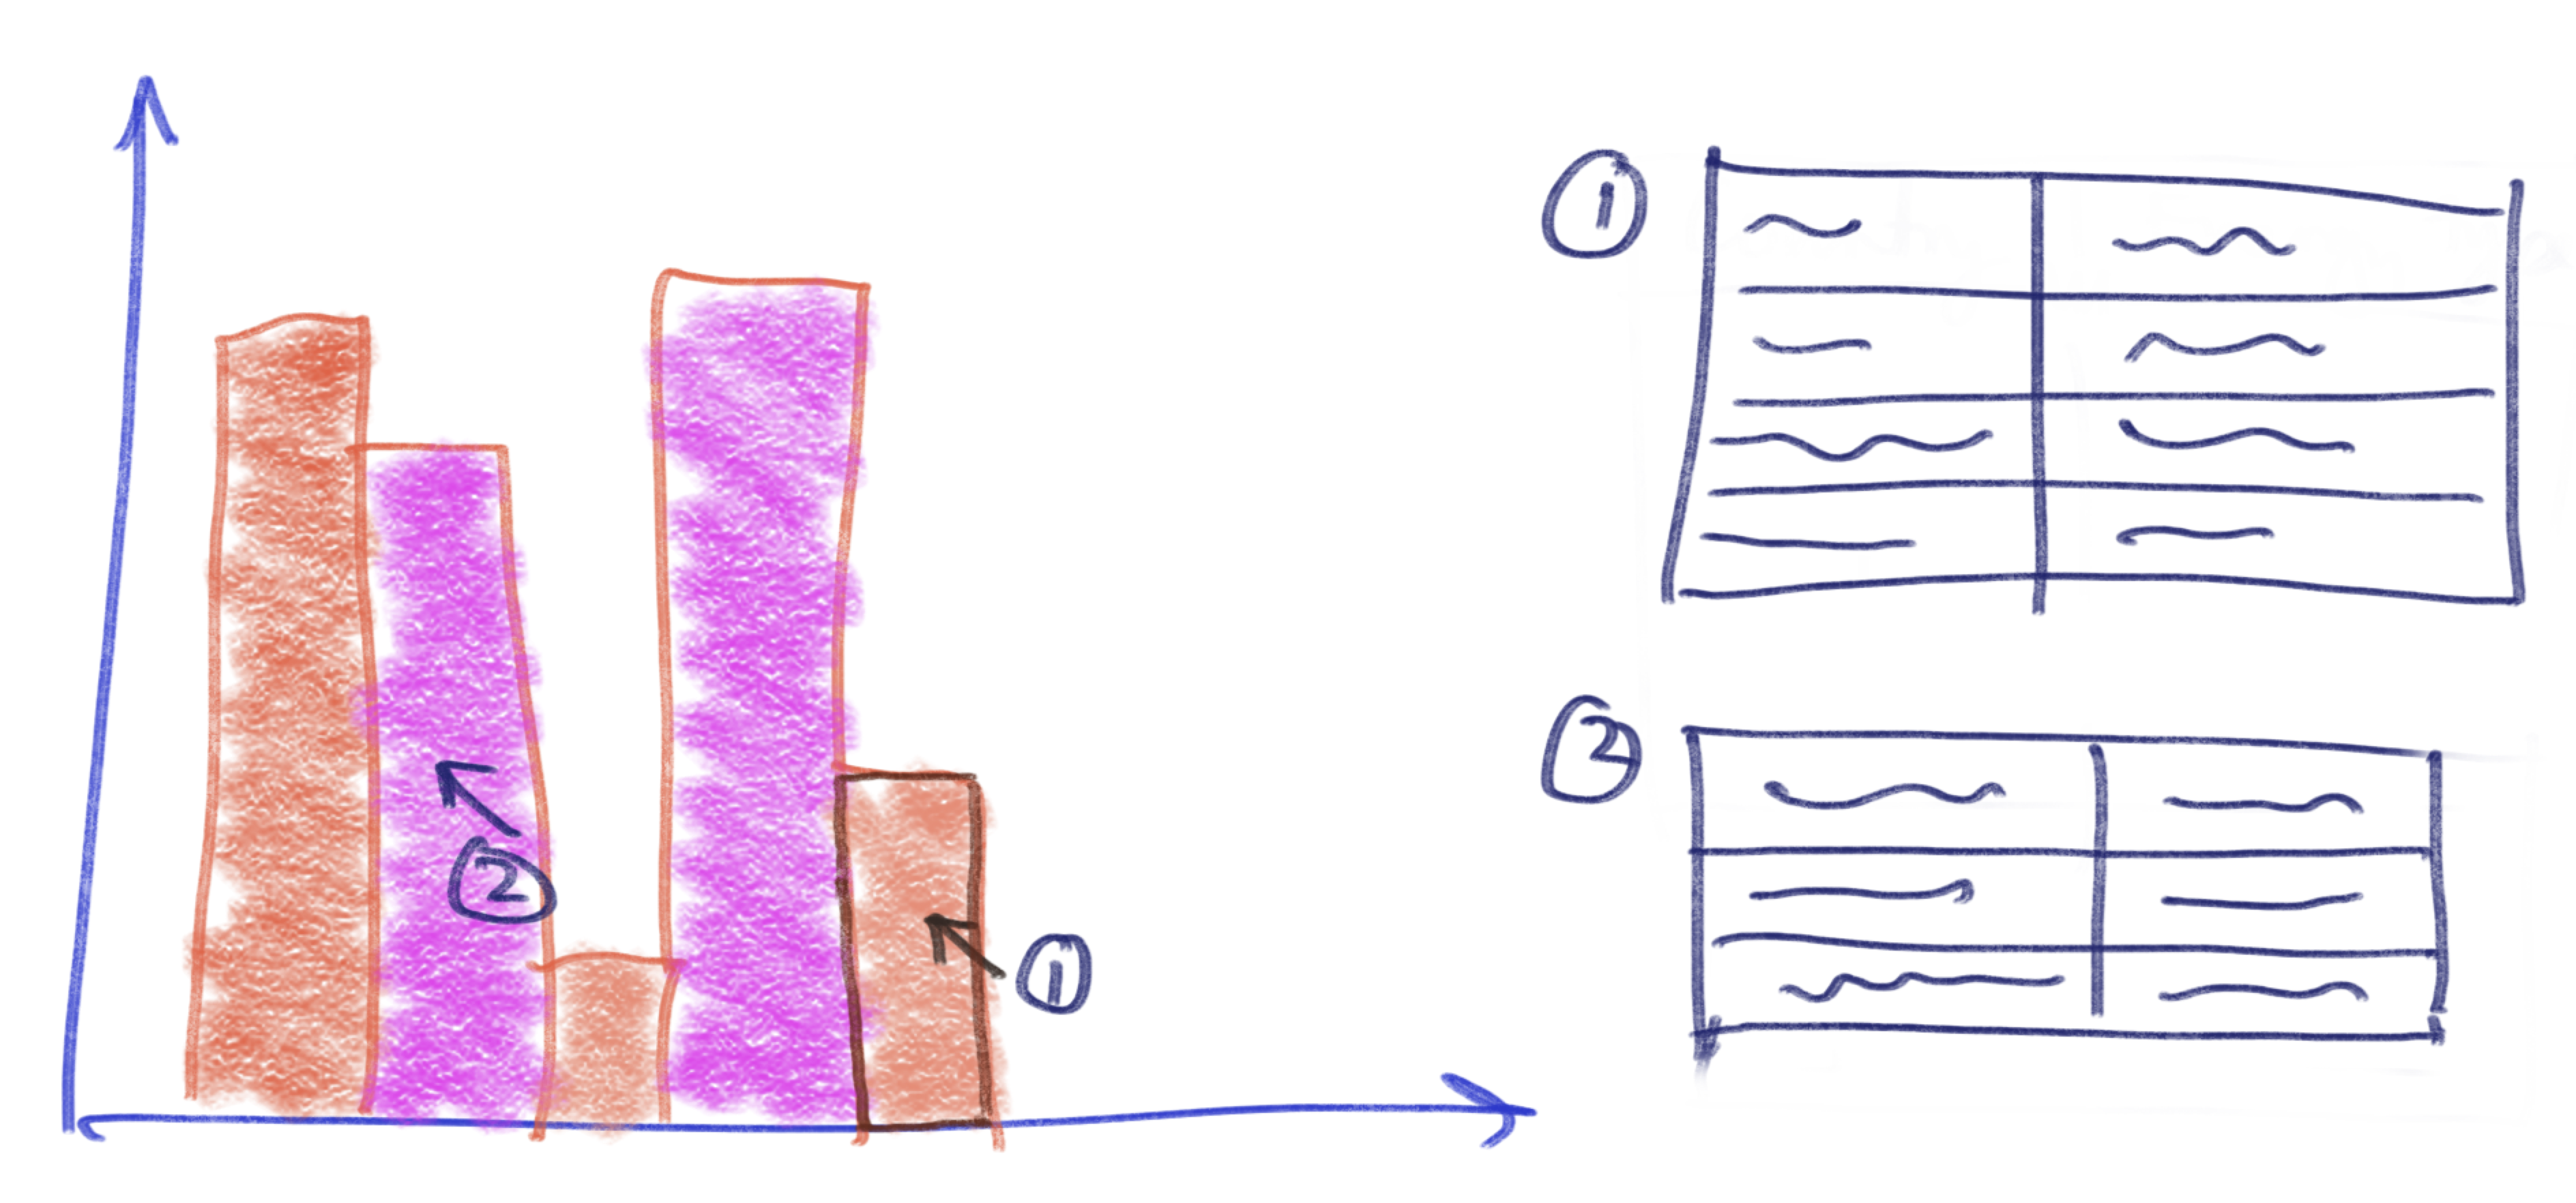
\includegraphics[scale=0.07]{fig/example/data-linking.png}}
   \caption{Data visualisation with fine-grained data linking}
   \label{fig:introduction:data-linking}
\end{figure}

Building this sort of ``data-linked'' visualisation by hand is possible, but is a significant undertaking, requiring intimate knowledge of the computational relationship between chart and data, and programming effort to expose that information to the reader. Manual approaches are also unlikely to be correct and lead to brittle solutions that need to be changed whenever the application logic changes. Given that a visualisation is a view computed from a data source, it seems plausible that we might adapt techniques from program analysis and data provenance to provide a runtime infrastructure that automatically supports linked selections. Then the data scientist or visualisation designer can concern themselves with cleaning, aggregating and presenting data, leaving the infrastructure to take care of linking visualisations to the underlying data sources.
